\documentclass[aspectratio=169]{beamer}
\usepackage{graphicx}
\usepackage{xcolor}
\usepackage{algorithm}
\usepackage[noend]{algpseudocode}
\usepackage{algorithmicx}
\usepackage[absolute,overlay]{textpos}
\usepackage{transparent}
\title{TOPOLOGICAL SORT}
\author{mahirlabibdihan}
\date{February 2023}

\usepackage{tikz}
\usetikzlibrary{automata, positioning}
\usetikzlibrary{positioning, calc}
\usetikzlibrary{arrows,shapes, arrows.meta}
\usetikzlibrary {automata} 
\usecolortheme{seahorse}
\usefonttheme{professionalfonts}
\beamertemplatenavigationsymbolsempty
\tikzstyle{arrow} = [ line width=1mm,->,-latex]
\algnewcommand\algorithmicforeach{\textbf{for each}}
\algdef{S}[FOR]{ForEach}[1]{\algorithmicforeach\ #1\ \algorithmicdo}
\tikzstyle{vertex}=[circle split,draw = black,thick, minimum size=30pt,inner sep=3pt, fill=brown!30, outer sep=2pt]
\tikzstyle{vertex2}=[circle,draw = black,thick, minimum size=20pt,inner sep=3pt,  fill=blue!30, outer sep=2pt]
\tikzstyle{vertex3}=[circle,draw = black,thick, minimum size=30pt,inner sep=3pt,  fill=brown!30, outer sep=2pt]
\tikzstyle{vertex4}=[circle,draw = black,thick, minimum size=15pt,inner sep=3pt,  fill=brown!30, outer sep=2pt]
\tikzstyle{vertex5}=[rectangle,draw = black,thick, minimum width=50, minimum height = 20, inner sep=3pt,  fill=brown!30, outer sep=2pt]

\tikzstyle{vertex6}=[rectangle,draw = black,thick, minimum width=28, minimum height = 15, inner sep=3pt,  fill=brown!30, outer sep=2pt, text width=18, align=center]
\tikzstyle{vertex7}=[ellipse,draw = black,thick, minimum width=50, minimum height = 20, inner sep=3pt,  fill=brown!30, outer sep=2pt]
\tikzstyle{vertex8}=[ellipse,draw = black,thick, minimum width=50, minimum height = 30, inner sep=3pt,  fill=brown!30, outer sep=2pt]
\tikzstyle{selected vertex} = [vertex, fill=red!50]
\tikzstyle{blue vertex} = [vertex, fill=blue!24]
\tikzstyle{edge} = [draw,thick,-]
\tikzstyle{weight} = [font=\small]
\tikzstyle{selected edge} = [draw,line width=5pt,-,red!50]
\tikzstyle{ignored edge} = [draw,line width=5pt,-,black!20]
\tikzstyle{greenrect} = [rectangle, minimum width=0.5cm, minimum height=5cm, draw=white, fill=white]

\tikzstyle{active edge} =[draw,->, line width=3pt, orange]
\tikzstyle{inactive edge}=[draw,->, line width=2pt, black!50]
\tikzstyle{normal edge}=[draw,->, line width=2pt, black]

\tikzstyle{active node} = [circle, draw=black, thick, minimum size=20pt,inner sep=3pt,  fill=yellow!50, outer sep=2pt ]
\tikzstyle{active node2} = [circle, draw=black, thick, minimum size=20pt,inner sep=3pt,  fill=green!50, outer sep=2pt]
\tikzstyle{inactive node} = [circle, draw=black!50, thick, minimum size=20pt,inner sep=3pt,  outer sep=2pt]
\tikzstyle{normal node} = [circle, draw=black, thick, minimum size=20pt,inner sep=3pt, outer sep=2pt ]
\tikzstyle{listed node} = [circle, draw=black, thick, minimum size=20pt,inner sep=3pt,  fill=blue!50, outer sep=2pt]





\setbeamercolor{itemize item}{fg=black}
% \defbeamertemplate{itemize item}{\blacksquare}{}
% \setbeamertemplate{itemize items}[\blacksquare]

\begin{document}
\setbeamercolor{background canvas}{bg=black}
\begin{frame}{}
\begin{tikzpicture}
    \draw[color=white,fill=white,transform canvas={xshift = 5cm, yshift=-0.5cm}] (0,0) rectangle (0.2,3);
\end{tikzpicture}
\begin{textblock}{5}(6.5,6.8)
\fontfamily{qhv}\selectfont
\LARGE\color{white} \textbf{TOPOLOGICAL\\ SORT}
\end{textblock}
\begin{textblock}{5.6}(0,6.8)
    \fontfamily{qcr}\selectfont
    \small
    \color{white}
    \hfill Sayem Shahad Soummo \\ 
    \hfill Mahir Labib Dihan \\ 
    \hfill Souvik Ghosh \\
\end{textblock}
\end{frame}
\input{Page/Introduction.tex}
\setbeamercolor{background canvas}{bg=white}
\color{black}


\begin{frame}
    \transfade
    
\begin{textblock}{14}(1,2)
\begin{itemize}
        \item<1-> 
        For every edge in a DAG, the starting vertex is visited before ending vertex..
\end{itemize}
\end{textblock}


\begin{textblock}{16}(0,4)
    \begin{figure}
    \centering
    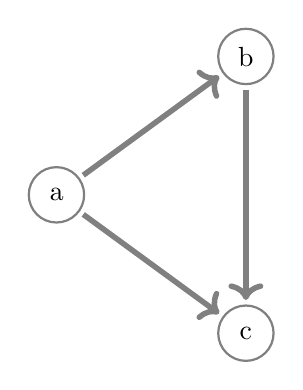
\begin{tikzpicture}
    \node<2> (a) [inactive node] {a} ;
    \node<2> (b) [inactive node, right of = a, xshift = 40, yshift = 50] {b};
    \node<2> (c) [inactive node, right of = a, xshift = 40, yshift = -50] {c};
    
    \draw<2> [inactive edge] (a) -- (b);
    \draw<2> [inactive edge] (a) -- (c);
    \draw<2> [inactive edge] (b) -- (c);
    
    \end{tikzpicture}
\end{figure}
\end{textblock}






   
\end{frame}
\begin{frame}
    \transfade
    \input{Simulation_sayem/definition_2}
   
\end{frame}
\begin{frame}
    \transfade
    \begin{textblock}{14}(1,2)
\begin{itemize}
        \item<1-> 
        For every edge in a DAG, the starting vertex is visited before ending vertex..
\end{itemize}
\end{textblock}


\begin{textblock}{16}(0,4)
    \begin{figure}
    \centering
    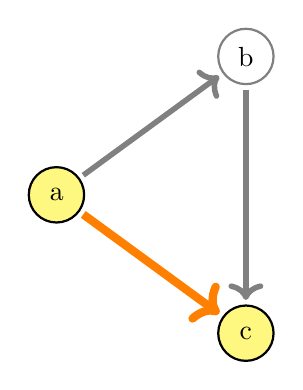
\begin{tikzpicture}
    \node<1-> (a) [active node] {a} ;
    \node<1-> (b) [inactive node, right of = a, xshift = 40, yshift = 50] {b};
    \node<1-> (c) [active node, right of = a, xshift = 40, yshift = -50] {c};
    
    \draw<1-> [inactive edge] (a) -- (b);
    \draw<1-> [active edge] (a) -- (c);
    \draw<1-> [inactive edge] (b) -- (c);
    
    \end{tikzpicture}
\end{figure}
\end{textblock}


\begin{textblock}{14}(1,9)
    \begin{itemize}
        \item<2> a is visited before c 
    \end{itemize}
    
\end{textblock}
   
\end{frame}
\begin{frame}
    \transfade
    \begin{textblock}{14}(1,2)
\begin{itemize}
        \item<1-> 
        For every edge in a DAG, the starting vertex is visited before ending vertex..
\end{itemize}
\end{textblock}


\begin{textblock}{16}(0,4)
    \begin{figure}
    \centering
    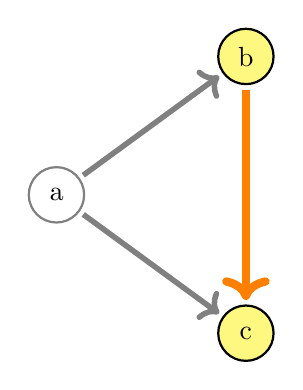
\begin{tikzpicture}
    \node<1-> (a) [inactive node] {a} ;
    \node<1-> (b) [active node, right of = a, xshift = 40, yshift = 50] {b};
    \node<1-> (c) [active node, right of = a, xshift = 40, yshift = -50] {c};
    
    \draw<1-> [inactive edge] (a) -- (b);
    \draw<1-> [inactive edge] (a) -- (c);
    \draw<1-> [active edge] (b) -- (c);
    
    \end{tikzpicture}
\end{figure}
\end{textblock}


\begin{textblock}{14}(1,9)
    \begin{itemize}
        \item<2> b is visited before c 
    \end{itemize}
    
\end{textblock}
   
\end{frame}

\input{Page/Example}

\begin{frame}
    
    \transfade
   
    \begin{textblock}{16}(0,7)
        \centering
        \color{black}
        \Huge \textbf{Let's assemble a PC!!!}
    \end{textblock}
   
    
\end{frame}

\begin{frame}
    \transfade
    \color{black}



\begin{textblock}{16}(0,2)

\begin{figure}
    \centering
    \begin{tikzpicture}

\node[inner sep=0pt] (motherboard) at (3,0)
    {\includegraphics[width=.12\textwidth]{Simulation_sayem/pictures/motherboard.png}};  
\node[inner sep=0pt] (videocard) at (3,3)
    {\includegraphics[width=.12\textwidth]{Simulation_sayem/pictures/video-card.png}};
    
\node[inner sep=0pt] (memory) at (0,0)
    {\includegraphics[width=.12\textwidth]{Simulation_sayem/pictures/memory.png}};
    
\node[inner sep=0pt] (casing) at (6,0)
    {\includegraphics[width=.12\textwidth]{Simulation_sayem/pictures/casing.jpg}};
\node[inner sep=0pt] (PSU) at (6,3)
    {\includegraphics[width=.12\textwidth]{Simulation_sayem/pictures/powerSupply.jpg}};
\node[inner sep=0pt] (CPU) at (0,3) {\includegraphics[width=.08\textwidth]{Simulation_sayem/pictures/processor.jpg}};


\node<3>[inner sep=0pt] (casingcross) at (6,0)
    {\includegraphics[width=.12\textwidth]{Simulation_sayem/pictures/cross.png}};
\node<6>[inner sep=0pt] (memorycross) at (0,0)
    {\includegraphics[width=.12\textwidth]{Simulation_sayem/pictures/cross.png}};


\draw<4-> [inactive edge] (PSU) --(casing);
\draw<4-> [inactive edge] (motherboard) --(casing);
\draw<10-> [inactive edge] (videocard) --(PSU);
\draw<8-> [inactive edge] (motherboard) --(videocard);
\draw<8-> [inactive edge] (CPU) --(videocard);
\draw<9-> [inactive edge] (motherboard) --(CPU);
\draw<7-> [inactive edge] (motherboard) --(memory);

\end{tikzpicture}
\end{figure}
\end{textblock}

\begin{textblock}{14}(5,12)
\begin{figure}
    \centering
    \begin{itemize}
        \only<2>{
        \vfill \item<2> Lets buy casing first }
        \only<3>{
        \vfill \item<3> But we can't!! }
        \only<4>{
        \vfill \item<4> We need motherboard and PSU model }
        \only<5>{
        \vfill \item<5> Lets try to buy RAM }
        \only<6>{
        \vfill \item<6> Again!! We can't }
        \only<7>{
        \vfill \item<7> We need motherboard model }
    \end{itemize}
\end{figure}
    
\end{textblock}
\end{frame}

\begin{frame}
    \transfade
    \begin{itemize}
        \item<1-> We can't buy things in random order
        \item<2-> Maintain the topological Order!!!
        
    \end{itemize}

\end{frame}

\begin{frame}
    \transfade
    \begin{textblock}{16}(0,6)
        \centering
        \color{black}
        \Large \textbf{Let's get back to our example}
    \end{textblock}
    
\end{frame}


\begin{frame}
    \transfade
    
\begin{textblock}{16}(0,2)
\begin{figure}
    \centering
    \begin{tikzpicture}

\node<1->[inner sep=0pt] (motherboard) at (3,0)
    {\includegraphics[width=.12\textwidth]{Simulation_sayem/pictures/motherboard.png}};  
\node<1->[inner sep=0pt] (videocard) at (3,3)
    {\includegraphics[width=.12\textwidth]{Simulation_sayem/pictures/video-card.png}};
    
\node<1->[inner sep=0pt] (memory) at (0,0)
    {\includegraphics[width=.12\textwidth]{Simulation_sayem/pictures/memory.png}};
    
\node<1->[inner sep=0pt] (casing) at (6,0)
    {\includegraphics[width=.12\textwidth]{Simulation_sayem/pictures/casing.jpg}};
\node<1->[inner sep=0pt] (PSU) at (6,3)
    {\includegraphics[width=.12\textwidth]{Simulation_sayem/pictures/powerSupply.jpg}};
\node<1->[inner sep=0pt] (CPU) at (0,3)
    {\includegraphics[width=.08\textwidth]{Simulation_sayem/pictures/processor.jpg}};


\node<2->[inner sep=0pt] (motherboardtik) at (3,0)
    {\includegraphics[width=.09\textwidth]{Simulation_sayem/pictures/tik.png}};
\node<3->[inner sep=0pt] (CPUtik) at (0,3)
    {\includegraphics[width=.09\textwidth]{Simulation_sayem/pictures/tik.png}};
\node<4->[inner sep=0pt] (videocardtik) at (3,3)
    {\includegraphics[width=.09\textwidth]{Simulation_sayem/pictures/tik.png}};
\node<5->[inner sep=0pt] (PSUtik) at (6,3)
    {\includegraphics[width=.09\textwidth]{Simulation_sayem/pictures/tik.png}};
\node<6->[inner sep=0pt] (casingtik) at (6,0)
    {\includegraphics[width=.09\textwidth]{Simulation_sayem/pictures/tik.png}};
\node<7->[inner sep=0pt] (memorytik) at (0,0)
    {\includegraphics[width=.09\textwidth]{Simulation_sayem/pictures/tik.png}};

\draw<1-> [inactive edge] (videocard) --(PSU);
\draw<1-> [inactive edge] (motherboard) --(videocard);
\draw<1-> [inactive edge] (CPU) --(videocard);
\draw<1-> [inactive edge] (motherboard) --(CPU);
\draw<1-> [inactive edge] (PSU) --(casing);
\draw<1-> [inactive edge] (motherboard) --(casing);
\draw<1-> [inactive edge] (motherboard) --(memory);


\end{tikzpicture}
\end{figure}
\end{textblock}


\begin{textblock}{14}(1,11)
    \begin{itemize}
        \item<2-> Our shopping list
    \end{itemize}
\end{textblock}


\begin{textblock}{14}(2.5,12)
    
    
    \begin{tikzpicture}

\node<2->[inner sep=0pt] (motherboard) at (0,0)
    {\includegraphics[width=.10\textwidth]{Simulation_sayem/pictures/motherboard.png}};  
\node<4->[inner sep=0pt] (videocard) at (4,0)
    {\includegraphics[width=.10\textwidth]{Simulation_sayem/pictures/video-card.png}};
    
\node<7->[inner sep=0pt] (memory) at (10,0)
    {\includegraphics[width=.10\textwidth]{Simulation_sayem/pictures/memory.png}};
    
\node<6->[inner sep=0pt] (casing) at (8,0)
    {\includegraphics[width=.073\textwidth]{Simulation_sayem/pictures/casing.jpg}};
\node<5->[inner sep=0pt] (PSU) at (6,0)
    {\includegraphics[width=.10\textwidth]{Simulation_sayem/pictures/powerSupply.jpg}};
\node<3->[inner sep=0pt] (CPU) at (2,0)
    {\includegraphics[width=.06\textwidth]{Simulation_sayem/pictures/processor.jpg}};



\end{tikzpicture}

\end{textblock} 
\end{frame}


\begin{frame}
    \transfade
    

\begin{textblock}{14}(2,3)
    \begin{itemize}
    \item<1-> There can exist multiple ordering
\end{itemize}
\end{textblock}




\begin{textblock}{14}(2.5,4)
    
    
\begin{tikzpicture}

\node<2->[inner sep=0pt] (motherboard) at (0,0)
    {\includegraphics[width=.10\textwidth]{Simulation_sayem/pictures/motherboard.png}};  
\node<2->[inner sep=0pt] (videocard) at (6,0)
    {\includegraphics[width=.10\textwidth]{Simulation_sayem/pictures/video-card.png}};
    
\node<2->[inner sep=0pt] (memory) at (2,0)
    {\includegraphics[width=.10\textwidth]{Simulation_sayem/pictures/memory.png}};
    
\node<2->[inner sep=0pt] (casing) at (10,0)
    {\includegraphics[width=.10\textwidth]{Simulation_sayem/pictures/casing.jpg}};
\node<2->[inner sep=0pt] (PSU) at (8,0)
    {\includegraphics[width=.10\textwidth]{Simulation_sayem/pictures/powerSupply.jpg}};
\node<2->[inner sep=0pt] (CPU) at (4,0)
    {\includegraphics[width=.06\textwidth]{Simulation_sayem/pictures/processor.jpg}};

\end{tikzpicture}

\end{textblock}


\begin{textblock}{14}(2,7)
    \begin{itemize}
        \item[]<2->RAM can be bought right after motherboard
    \end{itemize}
    

\end{textblock}




\begin{textblock}{14}(2,9)
    \begin{itemize}
    \item<3-> Dependencies should be taken care beforehand \\
    In our example, we could not buy casing before motherboard and PSU
\end{itemize}
\end{textblock}

    
\end{frame}



\begin{frame}
    \transfade
    \begin{textblock}{16}(0,7.5)
        \centering
        \color{black}
        \Large \textbf{We have used topological sorting. But how it works!!!}
    \end{textblock}
    
\end{frame}





% \begin{frame}{}
%     \transboxin
    
%     \begin{itemize}
%         \item[$\blacksquare$] Topological sort is a graph traversal in which each node is visited only after all its dependencies are visited. \underline{If there is an edge from node u to v, then v is dependent on u}  \href{https://www.interviewcake.com/concept/java/topological-sort}{\underline{Link}} \pause
%         \item[$\blacksquare$] We can view a topological sort of a graph as an ordering of its vertices along a horizontal line so that all directed edges go from left to right. Topological sorting is thus different from the usual kind of “sorting”
%         \item[$\blacksquare$] In order to have a topological sorting, the graph must not contain any cycles and it must be directed i.e. the graph must be a DAG. \pause
%         \item[$\blacksquare$] There can be more than one topological sorting for a graph. \pause
%     \end{itemize}    
% \end{frame}

\input{Page/Simulation.tex}
\setbeamercolor{background canvas}{bg=white}

\begin{frame}{}
    \transfade
    \begin{frame}{}
\transfade
    \begin{textblock}{15}(1,2)
    \begin{itemize}
        \item[$\blacksquare$] Detecting cycle in a graph.
    \end{itemize}
    \end{textblock}
    \begin{textblock}{16}(0,3)
    \setbeamercovered{transparent}
    \begin{figure}
        \centering
        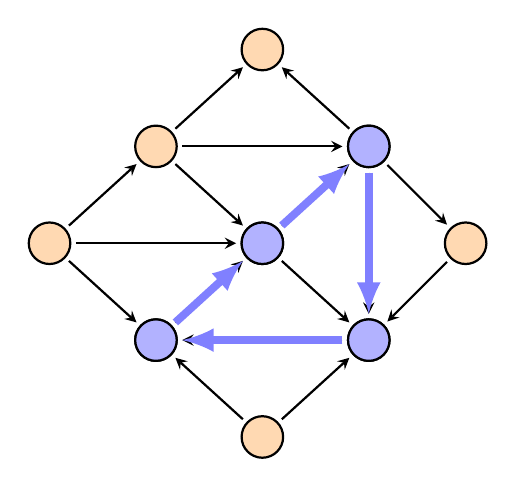
\begin{tikzpicture}[->, thick, >=stealth]
            \node(A) [vertex4, fill=orange!30]  {};
            \node(B) [vertex4, right of = A, xshift = 10, yshift =  35, fill=orange!30] {};
            \node<1>(C) [vertex4, right of = A, xshift = 10, yshift = -35, fill=orange!30] {};
            \node<2>(C) [vertex4, right of = A, xshift = 10, yshift = -35, fill=blue!30] {};
            \node<1>(D) [vertex4, right of = C, xshift = 10, yshift =  35, fill=orange!30] {};
            \node<2>(D) [vertex4, right of = C, xshift = 10, yshift =  35, fill=blue!30] {};
            \node<1>(E) [vertex4, right of = D, xshift = 10, yshift =  35, fill=orange!30] {};
            \node<2>(E) [vertex4, right of = D, xshift = 10, yshift =  35, fill=blue!30] {};
            \node<1>(F) [vertex4, right of = D, xshift = 10, yshift = -35, fill=orange!30] {};
            \node<2>(F) [vertex4, right of = D, xshift = 10, yshift = -35, fill=blue!30] {};
            \node(G) [vertex4, right of = B, xshift = 10, yshift = 35, fill=orange!30] {};
            \node(H) [vertex4, right of = C, xshift = 10, yshift = -35, fill=orange!30] {};
            \node(I) [vertex4, right of = D, xshift = 45, yshift = 0, fill=orange!30] {};

            \draw (A) -- (B);
            \draw (A) -- (C);
            \draw (A) -- (D);
            \draw (B) -- (D);
            \draw (B) -- (E);
            \draw<1> (C) -- (D);
            \draw<2> [arrow,blue!50] (C) -- (D);
            \draw<1> (F) -- (C);
            \draw<2> [arrow,blue!50] (F) -- (C);            
            \draw<1> (D) -- (E);
            \draw<2> [arrow,blue!50] (D) -- (E);
            \draw (D) -- (F);
            \draw<1> (E) -- (F);
            \draw<2> [arrow,blue!50] (E) -- (F);
            \draw (B) -- (G);
            \draw (E) -- (G);
            \draw (E) -- (I);
            \draw (I) -- (F);
            \draw (H) -- (C);
            \draw (H) -- (F);
            
            
            
        \end{tikzpicture}
    \end{figure}
\end{textblock}


\end{frame}

\end{frame}
\begin{frame}{}
    \transfade
    \documentclass{beamer}
\usetheme{Madrid}
\usepackage[utf8]{inputenc}

\title{Beamer}
\author{mahirlabibdihan }
\date{December 2022}
\title{Title}
\author{Author}
\institute{Institute}
\date{\today}

\AtBeginSection[]
{

}

\begin{document}
\frame{\titlepage}
\begin{frame}{Table of contents}
    \tableofcontents
\end{frame}
\begin{frame}{Frame 1}
\section{Introduction}
This is demo slide
\section{Section 2}
\section{Section 3}
\end{frame}
\end{document}

\end{frame}
\begin{frame}{}
    \transfade
    \begin{textblock}{14}(1,2)
\begin{itemize}
    \only<1> {
        \vfill \item[$\blacksquare$] Outgoing edges of node A also need to be removed which will decrease indegree of B,C,D by 1
    }
    \only<2> {
        \vfill \item[$\blacksquare$] Now Both B and C have indegree = 0. Select either one to be added to the topological ordering.
    }
\end{itemize}
\end{textblock}
\begin{textblock}{15}(0,3)
\begin{figure}
\centering
    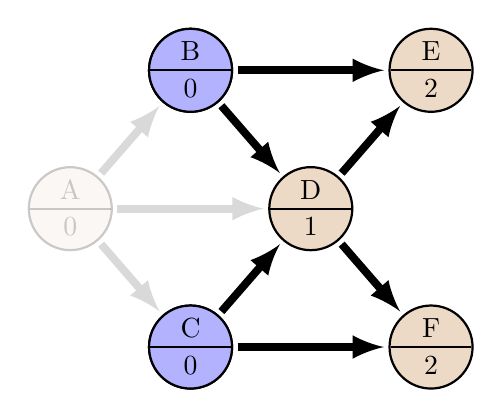
\begin{tikzpicture}
        \node(A) [vertex, opacity = 0.2]  {A \nodepart{lower} 0};
        \node(B) [vertex, right of = A, xshift = 15, yshift = 50] {B \nodepart{lower} 0};
        \node<2>(B) [vertex, right of = A, xshift = 15, yshift = 50, fill=blue!30] {B \nodepart{lower} 0};
        \node(C) [vertex, right of = A,xshift = 15, yshift = -50] {C \nodepart{lower} 0};
        \node<2>(C) [vertex, right of = A,xshift = 15, yshift = -50, fill=blue!30] {C \nodepart{lower} 0};
        \node(D) [vertex, right of = C, xshift = 15, yshift = 50] {D \nodepart{lower} 1};
        \node(E) [vertex, right of = D, xshift = 15, yshift = 50] {E \nodepart{lower} 2};
        \node(F) [vertex, right of = D, xshift = 15, yshift = -50] {F \nodepart{lower} 2};
        
        \draw [arrow, color = gray!30] (A) -- (B);
        \draw [arrow, color = gray!30] (A) -- (C);
        \draw [arrow, color = gray!30] (A) -- (D);
        \draw [arrow] (B) -- (D);
        \draw [arrow] (B) -- (E);
        \draw [arrow] (C) -- (D);
        \draw [arrow] (C) -- (F);
        \draw [arrow] (D) -- (E);
        \draw [arrow] (D) -- (F);
    \end{tikzpicture}
\end{figure}
\end{textblock}

\begin{textblock}{12}(1.3,12.5)
    \color{black}
    Topological\\Order
\end{textblock}

\begin{textblock}{12}(3.5,12.5)
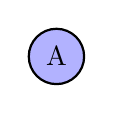
\begin{tikzpicture}
    \node(A) [vertex2,anchor=north] {A};
\end{tikzpicture}
\end{textblock}
\end{frame}
\begin{frame}{}
    \transfade
    \begin{figure}
    \centering
    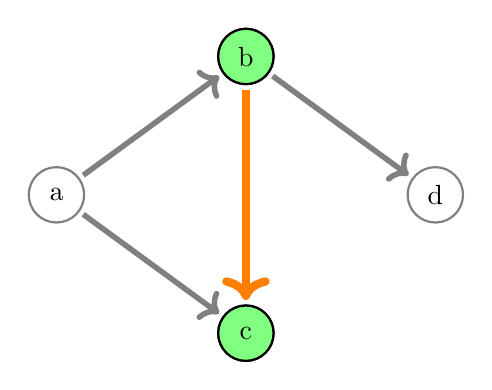
\begin{tikzpicture}
    \node (a) [inactive node] {a} ;
   
    \node (b) [active node, right of = a, xshift = 40, yshift = 50] {b};
    \node<2> (b) [active node2, right of = a, xshift = 40, yshift = 50] {b};
    
    \node (c) [active node, right of = a, xshift = 40, yshift = -50] {c};
    \node<4> (c) [active node2, right of = a, xshift = 40, yshift = -50] {c};
    
    \node (d) [inactive node, right of = b, xshift = 40, yshift = -50] {d};
    
    \draw [inactive edge] (a) -- (b);
    
    \draw [inactive edge] (a) -- (c);
    \draw [inactive edge] (b) -- (d);
    \draw [active edge] (b) -- (c);
    \end{tikzpicture}
\end{figure}

\begin{figure}
    \centering
    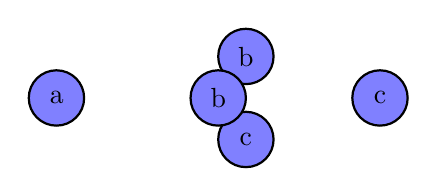
\begin{tikzpicture}
    \node<1-> (a) [listed node] {a} ;
    \node<1-4> (b1) [listed node, right of = a, xshift = 40,yshift=15] {b};
    \node<1-4> (c1) [listed node, right of = a, xshift = 40,yshift=-15] {c};
    \node<5> (b) [listed node, right of = a, xshift = 30] {b};
    \node<5> (c) [listed node, right of = b, xshift = 30] {c};
    \end{tikzpicture}
\end{figure}
\end{frame}
\begin{frame}{}
    \transfade
    \begin{figure}
    \centering
    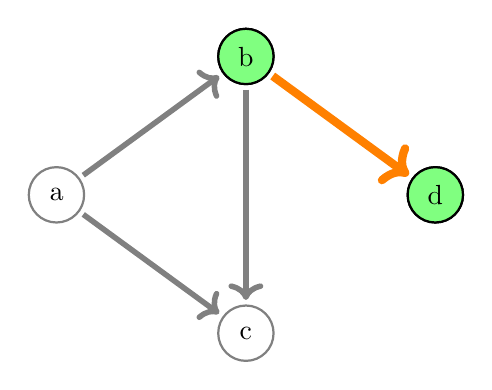
\begin{tikzpicture}
    \node (a) [inactive node] {a} ;
   
    \node (b) [active node, right of = a, xshift = 40, yshift = 50] {b};
    \node<2> (b) [active node2, right of = a, xshift = 40, yshift = 50] {b};
    
    \node (c) [inactive node, right of = a, xshift = 40, yshift = -50] {c};
   
    
    \node (d) [active node, right of = b, xshift = 40, yshift = -50] {d};
    \node<4> (d) [active node2, right of = b, xshift = 40, yshift = -50] {d};
    
    \draw [inactive edge] (a) -- (b);
    
    \draw [inactive edge] (a) -- (c);
    \draw [active edge] (b) -- (d);
    \draw [inactive edge] (b) -- (c);
    \end{tikzpicture}
\end{figure}

\begin{figure}
    \centering
    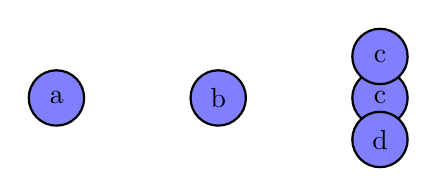
\begin{tikzpicture}
    \node<1-> (a) [listed node] {a} ;
    \node<1-> (b) [listed node, right of = a, xshift = 30] {b};
    \node<1-4> (c1) [listed node, right of = b, xshift = 30] {c};
    \node<5> (c) [listed node, right of = b, xshift = 30,yshift=15] {c};
    \node<5> (d) [listed node, right of = b, xshift = 30,yshift=-15] {d};
    \end{tikzpicture}
\end{figure}
\end{frame}
\begin{frame}{}
    \transfade
    \begin{textblock}{15}(1,2)
\begin{itemize}
    \only<1> {
        \vfill \item[$\blacksquare$] Add node D to the topological ordering and remove it from graph
    }
    \only<2> {
        \vfill \item[$\blacksquare$] Now Both E and F have indegree = 0. Select either to be added to the topological ordering.
    }
\end{itemize}
\end{textblock}
\begin{textblock}{15}(0,3)
\begin{figure}
\centering
    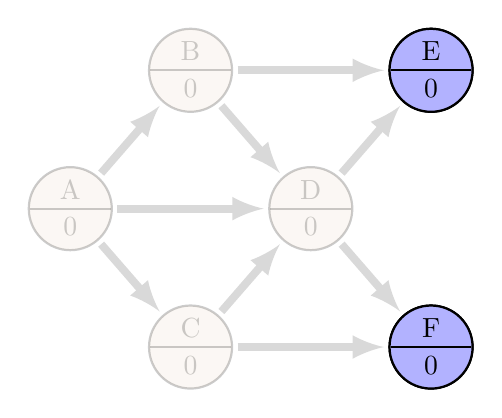
\begin{tikzpicture}
        \node(A) [vertex, opacity = 0.2]  {A \nodepart{lower} 0};
        \node(B) [vertex, opacity = 0.2, right of = A, xshift = 15, yshift = 50] {B \nodepart{lower} 0};
        \node(C) [vertex, opacity = 0.2, right of = A,xshift = 15, yshift = -50] {C \nodepart{lower} 0};
        \node(D) [vertex, opacity = 0.2,right of = C, xshift = 15, yshift = 50] {D \nodepart{lower} 0};
        \node(E) [vertex, right of = D, xshift = 15, yshift = 50] {E \nodepart{lower} 0};
        \node<2>(E) [vertex, right of = D, xshift = 15, yshift = 50, fill=blue!30] {E \nodepart{lower} 0};
        \node(F) [vertex, right of = D, xshift = 15, yshift = -50] {F \nodepart{lower} 0};
        \node<2>(F) [vertex, right of = D, xshift = 15, yshift = -50, fill=blue!30] {F \nodepart{lower} 0};
        
        \draw [arrow, color = gray!30] (A) -- (B);
        \draw [arrow, color = gray!30] (A) -- (C);
        \draw [arrow, color = gray!30] (A) -- (D);
        \draw [arrow, color = gray!30] (B) -- (D);
        \draw [arrow, color = gray!30] (B) -- (E);
        \draw [arrow, color = gray!30] (C) -- (D);
        \draw [arrow, color = gray!30] (C) -- (F);
        \draw [arrow, color = gray!30] (D) -- (E);
        \draw [arrow, color = gray!30] (D) -- (F);
    \end{tikzpicture}
\end{figure}
\end{textblock}

\begin{textblock}{12}(1.3,12.5)
    \color{black}
    Topological\\Order
\end{textblock}

\begin{textblock}{12}(3.5,12.5)
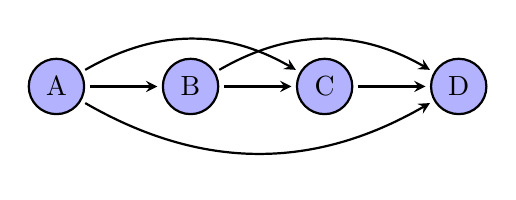
\begin{tikzpicture}[->, thick, >=stealth]
    \node(A) [vertex2] {A};
    \node(B) [vertex2, right of=A, xshift=20] {B};
    \node(C) [vertex2, right of=B, xshift=20] {C};
    \node(D) [vertex2, right of=C, xshift=20] {D};
    \path (A) edge [] node {} (B);
    \path (B) edge [] node {} (C);
    \path (A) edge [bend left] node {} (C);
    \path (C) edge [] node {} (D);
    \path (B) edge [bend left] node {} (D);
    \path (A) edge [bend right] node {} (D);
\end{tikzpicture}
\end{textblock}
\end{frame}
\begin{frame}{}
    \transfade
    \input{Simulation_dihan/6}
\end{frame}
\begin{frame}{}
    \transfade
    \begin{textblock}{15}(1,2)
\begin{itemize}
    \only<1> {
        \vfill \item[$\blacksquare$] Add node F to the topological ordering and remove it from graph
    }
\end{itemize}
\end{textblock}
\begin{textblock}{15}(0,3)
\begin{figure}
\centering
    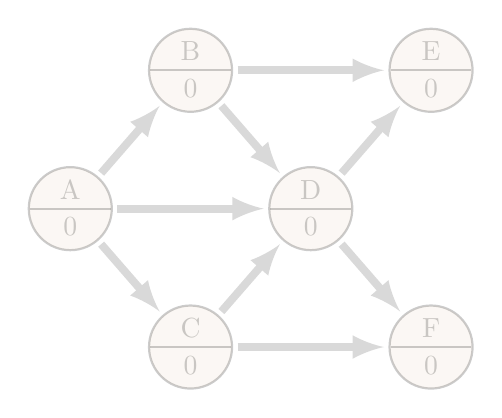
\begin{tikzpicture}
        \node(A) [vertex, opacity = 0.2]  {A \nodepart{lower} 0};
        \node(B) [vertex, opacity = 0.2, right of = A, xshift = 15, yshift = 50] {B \nodepart{lower} 0};
        \node(C) [vertex, opacity = 0.2, right of = A,xshift = 15, yshift = -50] {C \nodepart{lower} 0};
        \node(D) [vertex, opacity = 0.2,right of = C, xshift = 15, yshift = 50] {D \nodepart{lower} 0};
        \node(E) [vertex, opacity = 0.2, right of = D, xshift = 15, yshift = 50] {E \nodepart{lower} 0};
        \node(F) [vertex, opacity = 0.2, right of = D, xshift = 15, yshift = -50] {F \nodepart{lower} 0};
        
        \draw [arrow, color = gray!30] (A) -- (B);
        \draw [arrow, color = gray!30] (A) -- (C);
        \draw [arrow, color = gray!30] (A) -- (D);
        \draw [arrow, color = gray!30] (B) -- (D);
        \draw [arrow, color = gray!30] (B) -- (E);
        \draw [arrow, color = gray!30] (C) -- (D);
        \draw [arrow, color = gray!30] (C) -- (F);
        \draw [arrow, color = gray!30] (D) -- (E);
        \draw [arrow, color = gray!30] (D) -- (F);
    \end{tikzpicture}
\end{figure}
\end{textblock}

\begin{textblock}{12}(1.3,12.5)
    \color{black}
    Topological\\Order
\end{textblock}

\begin{textblock}{12}(3.5,12.5)
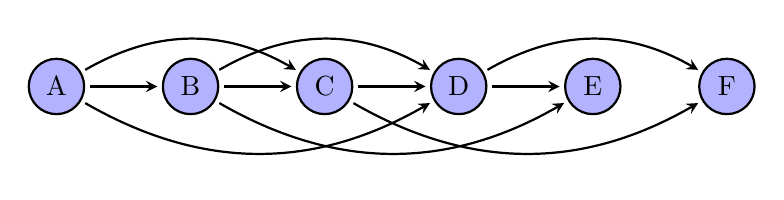
\begin{tikzpicture}[->, thick, >=stealth]
    \node(A) [vertex2] {A};
    \node(B) [vertex2, right of=A, xshift=20] {B};
    \node(C) [vertex2, right of=B, xshift=20] {C};
    \node(D) [vertex2, right of=C, xshift=20] {D};
    \node(E) [vertex2, right of=D, xshift=20] {E};
    \node(F) [vertex2, right of=E, xshift=20] {F};
    \path (A) edge [] node {} (B);
    \path (B) edge [] node {} (C);
    \path (A) edge [bend left] node {} (C);
    \path (C) edge [] node {} (D);
    \path (B) edge [bend left] node {} (D);
    \path (A) edge [bend right] node {} (D);
    \path (B) edge [bend right] node {} (E);
    \path (D) edge [] node {} (E);
    \path (D) edge [bend left] node {} (F);
    \path (C) edge [bend right] node {} (F);
\end{tikzpicture}
\end{textblock}
\end{frame}
\begin{frame}{}
    \transfade
    \begin{textblock}{15}(1,2)
    \begin{itemize}
        \only<1> {
        \vfill \item[$\blacksquare$] We have found the topological order
            }
    \end{itemize}
\end{textblock}

\begin{textblock}{6}(0,4.4)
    \setbeamercovered{transparent}
    \begin{figure}
        \centering
        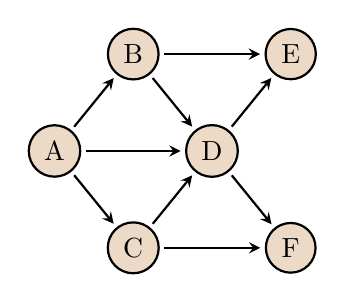
\begin{tikzpicture}[->, thick, >=stealth]
            \node<1>(A) [vertex4]  {A};
            \node(B) [vertex4, right of = A, xshift = 0, yshift =  35] {B};
            \node(C) [vertex4, right of = A, xshift = 0, yshift = -35] {C};
            \node(D) [vertex4, right of = C, xshift = 0, yshift =  35] {D};
            \node(E) [vertex4, right of = D, xshift = 0, yshift =  35] {E};
            \node(F) [vertex4, right of = D, xshift = 0, yshift = -35] {F};

            \draw (A) -- (B);
            \draw (A) -- (C);
            \draw (A) -- (D);
            \draw (B) -- (D);
            \draw (B) -- (E);
            \draw (C) -- (D);
            \draw (C) -- (F);
            \draw (D) -- (E);
            \draw (D) -- (F);
        \end{tikzpicture}
    \end{figure}

\end{textblock}

\begin{textblock}{3}(4.7,7.7)
    
\begin{tikzpicture}
        \draw [arrow] (0,0) -- (1,0);
    \end{tikzpicture}
\end{textblock}

\begin{textblock}{5}(2,11)
    \color{black} Unsorted Graph
\end{textblock}
\begin{textblock}{8}(8.3,11)
    Topologically Sorted Graph
\end{textblock}
\begin{textblock}{10}(5.5,6)
    \begin{figure}
        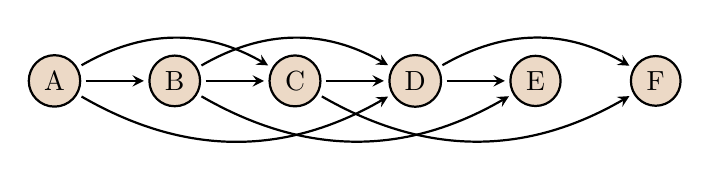
\begin{tikzpicture}[->, thick, >=stealth]
            \node(A) [vertex4] {A};
            \node(B) [vertex4, right of=A, xshift=15] {B};
            \node(C) [vertex4, right of=B, xshift=15] {C};
            \node(D) [vertex4, right of=C, xshift=15] {D};
            \node(E) [vertex4, right of=D, xshift=15] {E};
            \node(F) [vertex4, right of=E, xshift=15] {F};

            \path (A) edge [] node {} (B);
            \path (B) edge [] node {} (C);
            \path (A) edge [bend left] node {} (C);
            \path (C) edge [] node {} (D);
            \path (B) edge [bend left] node {} (D);
            \path (A) edge [bend right] node {} (D);
            \path (B) edge [bend right] node {} (E);
            \path (D) edge [] node {} (E);
            \path (D) edge [bend left] node {} (F);
            \path (C) edge [bend right] node {} (F);
        \end{tikzpicture}
    \end{figure}
\end{textblock}
\end{frame}

\begin{frame}{}
    \transcover
\end{frame}

\begin{frame}{}
    \transfade
    \begin{columns}
    \column{0.4\textwidth}
    \begin{itemize}
        \item<1->[$\blacksquare$] Kahn's Algorithm
        \item<2->[$\blacksquare$] BFS
        \item<3->[$\blacksquare$] {$O(|V|+|E|)$}
    \end{itemize}
    \column<1->{0.6\textwidth}
    \begin{algorithm}[H]
    % \algsetup{linenosize=\tiny}
    \begin{algorithmic}[1]
    \small
    \Procedure{TopoSort}{$G$} 
    \State create a list $L$
    \State create a queue $Q$
    \ForEach {vertex $v \in G$}
    \If{the indegree of $v = 0$}
    \State put v into the $Q$
    \EndIf
    \EndFor
    \While{$Q$ is not empty}
    \State pop a vertex v out of $Q$
    \State add v to the end of $L$
    \ForEach {edge $(u,v) \in G$}
    \State decrement the indegree of u
    \If{the indegree of $u = 0$}
    \State put u into the $Q$
    \EndIf
    \EndFor
    \EndWhile
    \State \Return $L$
    \EndProcedure
    \end{algorithmic}
\end{algorithm}
    \end{columns}
\end{frame}

\begin{frame}{}
    \transcover
\end{frame}

\begin{frame}{}
    \transfade
    \color{black}
    \begin{figure}
    \centering
        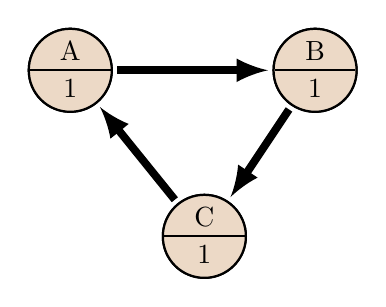
\begin{tikzpicture}
        \node<1-3> (A) [vertex3] {\Large A};
        \node<1-3> (B) [vertex3, right of = A,xshift = 60] {\Large B};
        \node<1-3> (C) [vertex3, right of = A,xshift =20, yshift=-60] {\Large C};
        
        \node<4> (A) [vertex] {A \nodepart{lower} 1};
        \node<4> (B) [vertex, right of = A,xshift = 60] {B \nodepart{lower} 1};
        \node<4> (C) [vertex, right of = A,xshift =20, yshift=-60] {C \nodepart{lower} 1};
        \draw [arrow] (A) -- (B);
        \draw [arrow] (B) -- (C);
        \draw [arrow] (C) -- (A);
    \end{tikzpicture}
    \end{figure}
    \begin{block}{}<2->
            \centering
            \Large What is the topological order?
    \end{block}
    \begin{block}{}<3->
            \centering
            \color{red}
            \Huge Not possible :(
    \end{block}
\end{frame}

\begin{frame}{}
    \transfade
    \Large
    \begin{block}{}<1->
        \centering
        Topological sorting is applicable for Directed Acyclic Graph (DAG). 
    \end{block}
    %  \begin{block}{}<2>
    %     \centering
    %     What's wrong with cyclic graphs? 
    % \end{block}
\end{frame}


\setbeamercolor{background canvas}{bg=black}
\begin{frame}{}
    \transcover
\begin{tikzpicture}
     \draw[color=white,fill=white,transform canvas={xshift = 5cm, yshift=-0.5cm}] (0,0) rectangle (0.2,3);
\end{tikzpicture}
\begin{textblock}{5}(6.5,7.3)
\fontfamily{qhv}\selectfont
\Huge\color{white} \textbf{WHERE?}
\end{textblock}
\end{frame}
\setbeamercolor{background canvas}{bg=white}
\begin{frame}{}
    \transuncover
\end{frame}

\setbeamercolor{background canvas}{bg=white}
\begin{frame}{}
\transfade
    \begin{textblock}{15}(1,2)
    \begin{itemize}
        \item[$\blacksquare$] Detecting cycle in a graph.
    \end{itemize}
    \end{textblock}
    \begin{textblock}{16}(0,3)
    \setbeamercovered{transparent}
    \begin{figure}
        \centering
        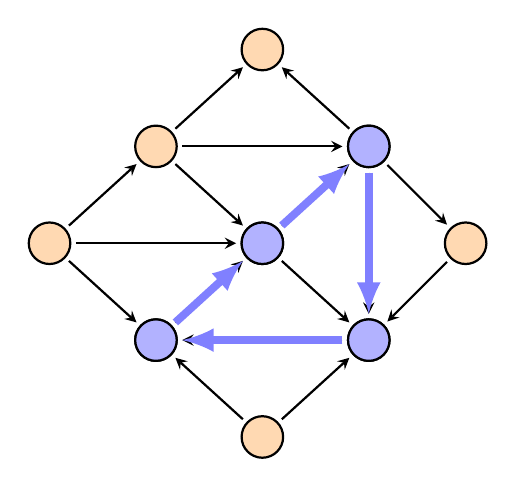
\begin{tikzpicture}[->, thick, >=stealth]
            \node(A) [vertex4, fill=orange!30]  {};
            \node(B) [vertex4, right of = A, xshift = 10, yshift =  35, fill=orange!30] {};
            \node<1>(C) [vertex4, right of = A, xshift = 10, yshift = -35, fill=orange!30] {};
            \node<2>(C) [vertex4, right of = A, xshift = 10, yshift = -35, fill=blue!30] {};
            \node<1>(D) [vertex4, right of = C, xshift = 10, yshift =  35, fill=orange!30] {};
            \node<2>(D) [vertex4, right of = C, xshift = 10, yshift =  35, fill=blue!30] {};
            \node<1>(E) [vertex4, right of = D, xshift = 10, yshift =  35, fill=orange!30] {};
            \node<2>(E) [vertex4, right of = D, xshift = 10, yshift =  35, fill=blue!30] {};
            \node<1>(F) [vertex4, right of = D, xshift = 10, yshift = -35, fill=orange!30] {};
            \node<2>(F) [vertex4, right of = D, xshift = 10, yshift = -35, fill=blue!30] {};
            \node(G) [vertex4, right of = B, xshift = 10, yshift = 35, fill=orange!30] {};
            \node(H) [vertex4, right of = C, xshift = 10, yshift = -35, fill=orange!30] {};
            \node(I) [vertex4, right of = D, xshift = 45, yshift = 0, fill=orange!30] {};

            \draw (A) -- (B);
            \draw (A) -- (C);
            \draw (A) -- (D);
            \draw (B) -- (D);
            \draw (B) -- (E);
            \draw<1> (C) -- (D);
            \draw<2> [arrow,blue!50] (C) -- (D);
            \draw<1> (F) -- (C);
            \draw<2> [arrow,blue!50] (F) -- (C);            
            \draw<1> (D) -- (E);
            \draw<2> [arrow,blue!50] (D) -- (E);
            \draw (D) -- (F);
            \draw<1> (E) -- (F);
            \draw<2> [arrow,blue!50] (E) -- (F);
            \draw (B) -- (G);
            \draw (E) -- (G);
            \draw (E) -- (I);
            \draw (I) -- (F);
            \draw (H) -- (C);
            \draw (H) -- (F);
            
            
            
        \end{tikzpicture}
    \end{figure}
\end{textblock}


\end{frame}


\begin{frame}{}
    \transcover
\end{frame}

\begin{frame}{}
\transfade
    \begin{textblock}{15}(1,2)
    \begin{itemize}
        \item[$\blacksquare$] Operation System deadlock detection.  
    \end{itemize}
    \end{textblock}
    \begin{textblock}{16}(0,4.4)
    \setbeamercovered{transparent}
    \begin{figure}
        \centering
        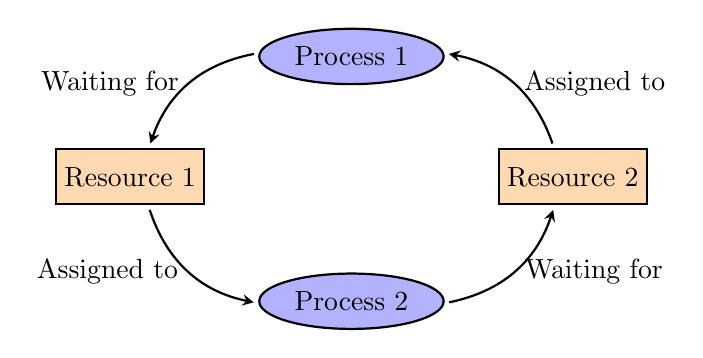
\begin{tikzpicture}[->, thick, >=stealth]
            \node(A) [vertex7, fill=blue!30]  {Process 1};
            \node(B) [vertex5, below of = A, xshift = -80, yshift = -15,fill=orange!30] {Resource 1};
            \node(C) [vertex5, below of = A, xshift = 80, yshift = -15,fill=orange!30] {Resource 2};
            \node(D) [vertex7, below of = A, xshift = 0, yshift = -60, fill=blue!30] {Process 2};
            
            
            \path (A) edge [bend right] node[anchor=east] {Waiting for} (B);
            \path (B) edge [bend right] node[anchor=east] {Assigned to} (D);
            \path (D) edge [bend right] node[anchor=west] {Waiting for} (C);
            \path (C) edge [bend right] node[anchor=west] {Assigned to} (A);
            
        \end{tikzpicture}
    \end{figure}
\end{textblock}
\end{frame}

\begin{frame}{}
    \transcover
\end{frame}

\begin{frame}{}
\transfade
    \begin{textblock}{15}(1,2)
    \begin{itemize}
        \item[$\blacksquare$] Course Schedule problem. 
    \end{itemize}
    \end{textblock}
    \begin{textblock}{16}(0,4)
    \setbeamercovered{transparent}
    \begin{figure}
        \centering
        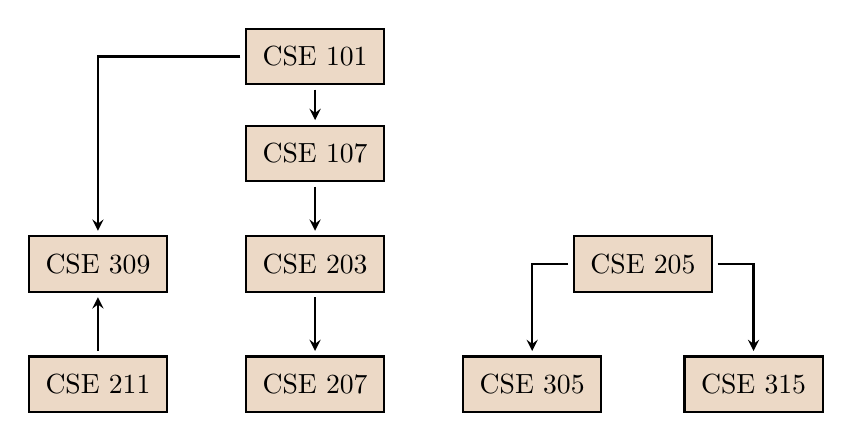
\begin{tikzpicture}[->, thick, >=stealth]
            \node(A) [vertex5]  {CSE 309};
            \node(B) [vertex5, below of = A, xshift = 0, yshift = -15] {CSE 211};
            \node(C) [vertex5, right of = A, xshift = 50, yshift =  75] {CSE 101};
            \node(D) [vertex5, right of = A, xshift = 50, yshift =  40] {CSE 107};
            \node(E) [vertex5, right of = A, xshift = 50, yshift =  0] {CSE 203};
            \node(F) [vertex5, below of = E, xshift = 0, yshift =  -15] {CSE 207};
            \node(G) [vertex5, right of = E, xshift = 90, yshift =  0] {CSE 205};
            \node(H) [vertex5, right of = F, xshift = 50, yshift =  0] {CSE 305};
            \node(I) [vertex5, right of = F, xshift = 130, yshift =  0] {CSE 315};

            \draw (B) -- (A);
            \draw (C) -| (A);
            \draw (C) -- (D);
            \draw (D) -- (E);
            \draw (E) -- (F);
            \draw (G) -| (H);
            \draw (G) -| (I);        
        
        \end{tikzpicture}

    \end{figure}
\end{textblock}
\end{frame}

\begin{frame}{}
    \transfade
    \begin{textblock}{15}(1,2)
        \begin{itemize}
            \item[$\blacksquare$] Course Schedule problem. 
        \end{itemize}
    \end{textblock}
    
    \begin{textblock}{16}(0,5.5)
    \centering
    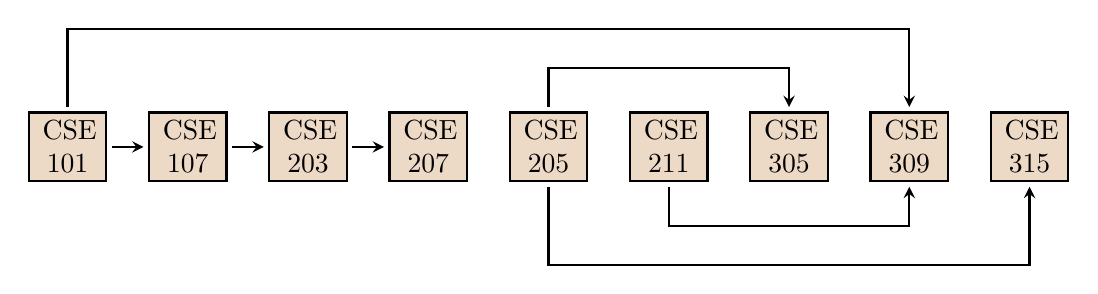
\begin{tikzpicture}[->, thick, >=stealth]
    \node(A) [vertex6]  {CSE 101};
    \node(B) [vertex6, right of = A, xshift = 15, yshift = 0] {CSE 107};
    \node(C) [vertex6, right of = B, xshift = 15, yshift =  0] {CSE 203};
    \node(D) [vertex6, right of = C, xshift = 15, yshift =  0] {CSE 207};
    \node(E) [vertex6, right of = D, xshift = 15, yshift =  0] {CSE 205};
    \node(F) [vertex6, right of = E, xshift = 15, yshift =  0] {CSE 211};
    \node(G) [vertex6, right of = F, xshift = 15, yshift =  0] {CSE 305};
    \node(H) [vertex6, right of = G, xshift = 15, yshift =  0] {CSE 309};
    \node(I) [vertex6, right of = H, xshift = 15, yshift =  0] {CSE 315}; 
    
    \draw (A) -- (B);
    \draw (B) -- (C);
    \draw (C) -- (D);
    \draw (A) --+ (0,1.5) -| (H);
    \draw (F) --+ (0,-1) -| (H);
    \draw (E) --+ (0,1) -| (G);
    \draw (E) --+ (0,-1.5) -| (I);
    \end{tikzpicture}
    \end{textblock}
\end{frame}


\begin{frame}{}
    \transcover
\end{frame}

\begin{frame}{}
\transfade
\begin{textblock}{16}(1,1.5)
    \begin{tikzpicture}

    \node<1->[inner sep=0pt] (b) at (0,4)
        {\includegraphics[width=.15\textwidth]{Simulation_souvik/Pictures/dependency.jpeg}};
    \node<1->[below of = b, yshift=-20]{Dependency resolution}; 
    
    \node<2->[inner sep=0pt] (f) at (5,4) {\includegraphics[width=.18\textwidth]{Simulation_souvik/Pictures/workflow.png}};
    \node<2->[below of = f, yshift=-20]{Manufacturing workflow};  
      
    \node<3->[inner sep=0pt] (e) at (10,4)
        {\includegraphics[width=.18\textwidth]{Simulation_souvik/Pictures/critical.jpeg}};
    \node<3->[below of = e, yshift=-20]{Critical path analysis};
    
    \node<4->[inner sep=0pt] (c) at (0,0.5)
        {\includegraphics[width=.18\textwidth]{Simulation_souvik/Pictures/sentance.jpeg}};
    \node<4->[below of = c, yshift=-15]{Sentence ordering};   
    
    \node<5->[inner sep=0pt] (a) at (5,0.5)
        {\includegraphics[width=.2\textwidth]{Simulation_souvik/Pictures/Task.png}};  
    \node<5->[below of = a, yshift=-15]{Task scheduling};
    
    \node<6->[inner sep=0pt] (d) at (10,0.5)
        {\includegraphics[width=.18\textwidth]{Simulation_souvik/Pictures/data.jpeg}};
    \node<6->[below of = d, yshift=-15]{Data serialization};
\end{tikzpicture}
\end{textblock}
\end{frame}


% \begin{frame}{}
%     \begin{itemize}
%         \item[$\blacksquare$] Single Source Shortest Path in a DAG. \pause
%         \item[$\blacksquare$] Dependency resolution.\pause
%         \item[$\blacksquare$] Sentence Ordering. \pause
%         \item[$\blacksquare$] Critical Path Analysis. \pause
%         \item[$\blacksquare$] Scheduling jobs from given dependencies among Jobs. For example, if some job requires the dependency of some other job, then we can use topological sorting. \pause
%         \item[$\blacksquare$] Other applications like manufacturing workflows, data serialization and context-free grammar. \pause
%     \end{itemize}
% \end{frame}

\input{Page/ThankYou.tex}
\end{document}
